\chapter{Results and Discussion}
\section{Major ion analysis}\label{sec:major_ion}
The products of the dissolution reaction of olivine in an open system at ambient conditions are shown in \Cref{eq:results_olivine}. 

\begin{equation} \label{eq:results_olivine}
\ce{(Mg_{0.94}Fe_{0.06})_{2}SiO_{4} + 4H_2O + 4CO_2 -> 1.88Mg^{+2} + 0.24Fe^{+2} + 4HCO_3^- + H_4SiO_4}
\end{equation}

\begin{figure}[h]
\centering
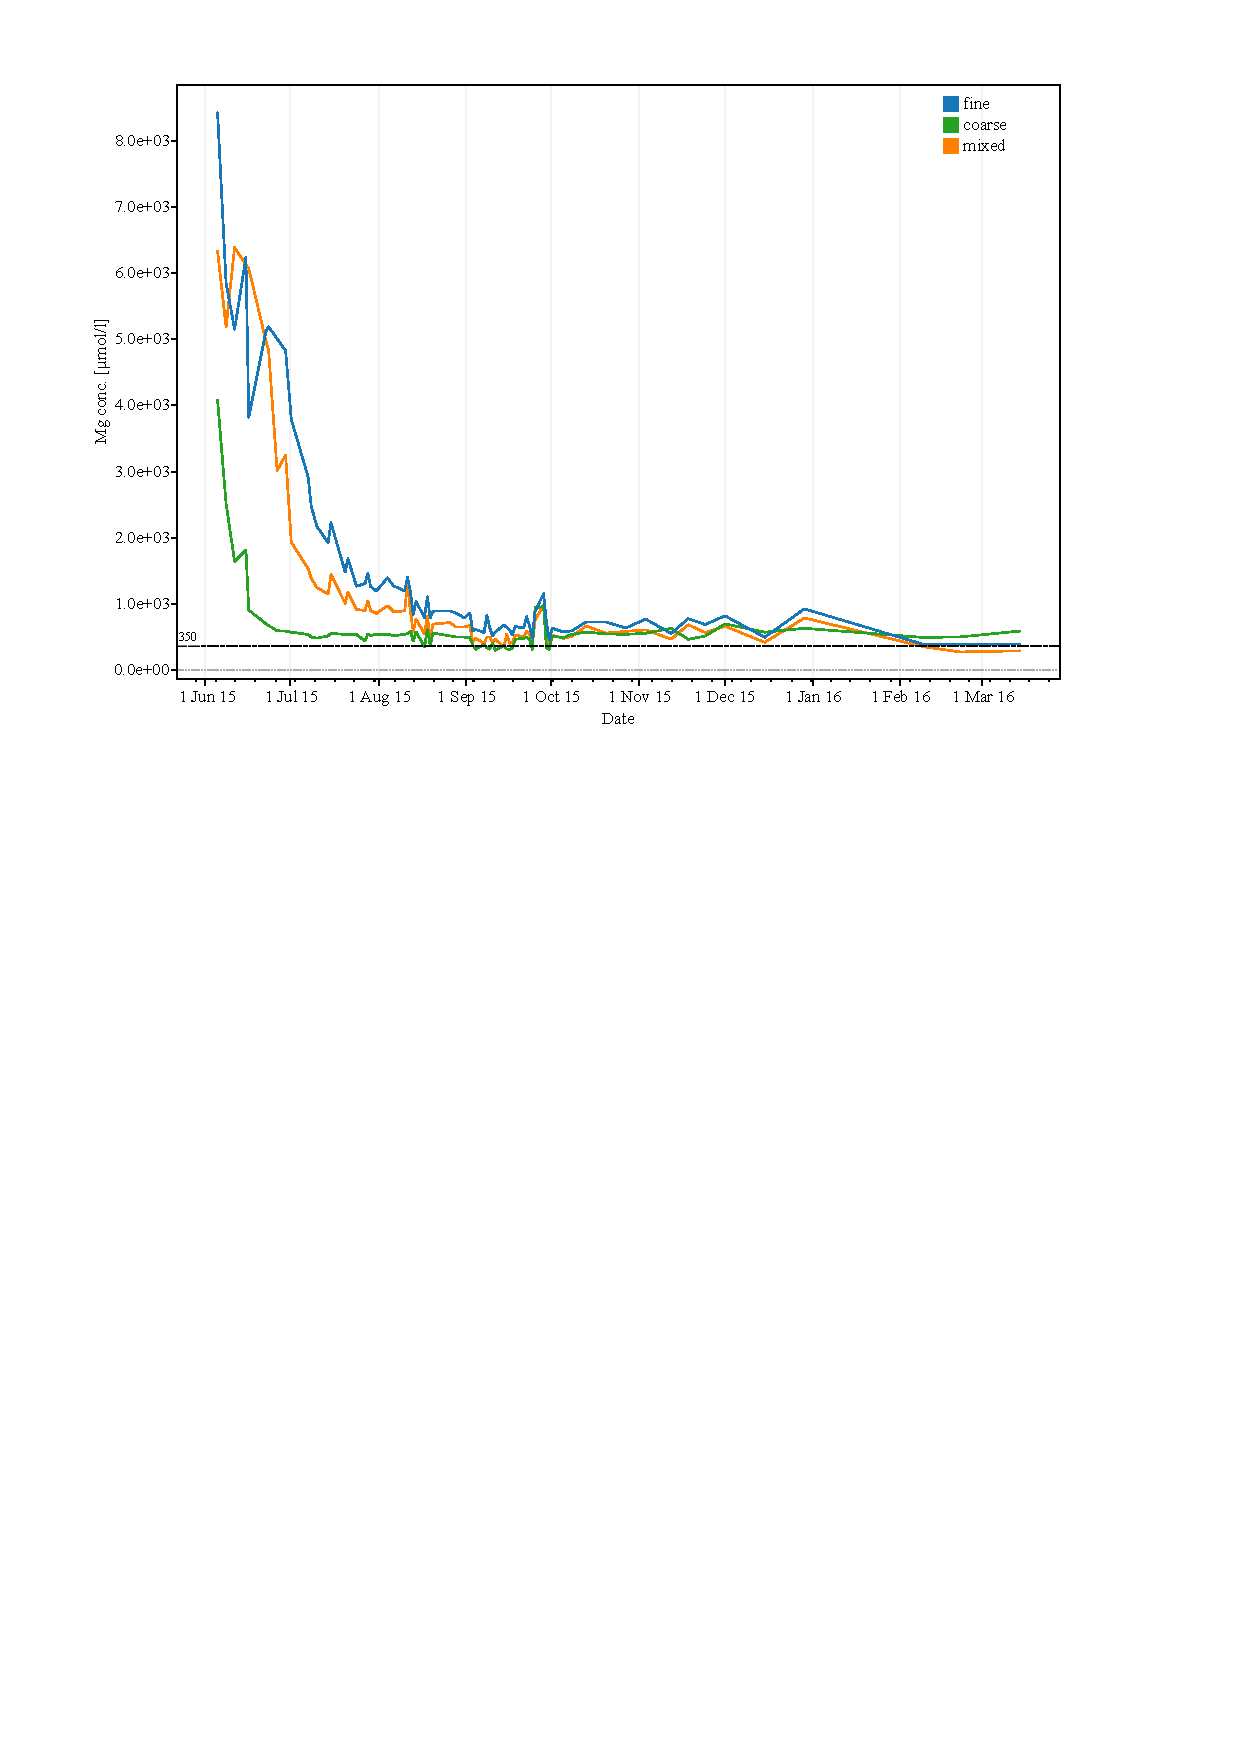
\includegraphics[scale=1]{mg.pdf}
\caption{The outlet [\ce{Mg^{+2}}] plotted against the Time (Date), averaged for the three grain types- fine, coarse, and mixed.}
\label{fig:results_mg1}
\end{figure}

\noindent \textbf{Mg:} The outlet /effluent concentration of Mg, in \si{\micro\mole\per\litre}, is plotted against time (date), with intervals of one month; averaged for each grain-type (\Cref{fig:results_mg1}). The concentration shows a power-law like decline for all three grain types. The fine and mixed release much more Mg than coarse in the first two months, the difference decreases over time and the pattern seems to show a slight reversal in the last month. The ratio of [\ce{Mg^{+2}}] in the outlet sample on the 30\textsuperscript{th} and 160\textsuperscript{th} day for fine : mixed : coarse is 8.2 : 5.5 : 1 and 1.5 : 1.2 : 1 respectively. The last measured value is around \SI{350}{\micro\mole\per\litre}.\\

\begin{figure}[h]
\centering
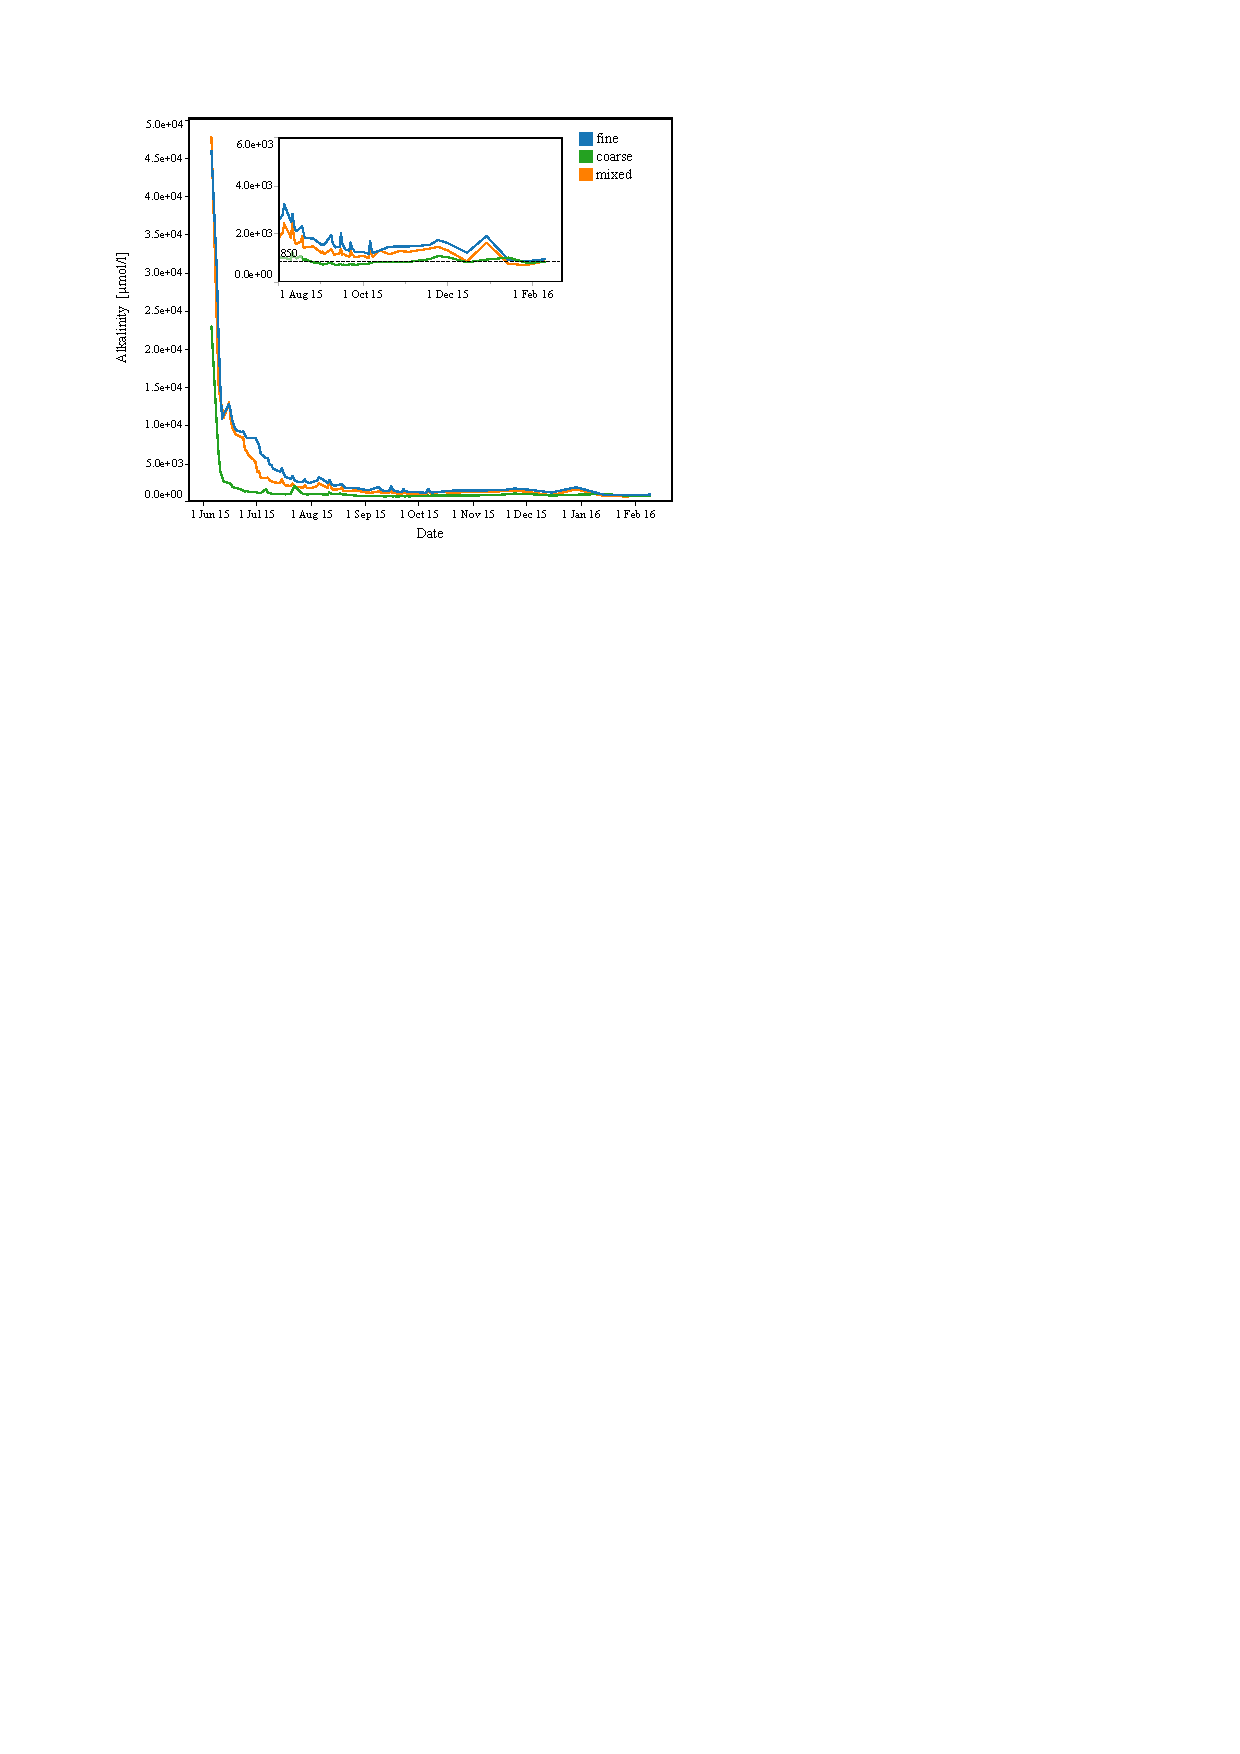
\includegraphics[scale=1.5]{alk.pdf}
\caption{The outlet Alkalinity plotted against Time (Date), averaged for the three grain types- fine, coarse, and mixed.}
\label{fig:results_alk}
\end{figure}

\noindent \textbf{Alkalinity:} The reaction\;\ref{eq:results_olivine} shows that the dissolved \ce{CO2} in the water appears as \ce{HCO_3^-} in the solution. The Alkalinity is defined as the amount of bases than turn to an uncharged species upon acid addition. In natural environments, total alkalinity can be substituted with carbonate alkalinity which constitutes carbonate (\ce{CO_3^{2-}}) and bicarbonate (\ce{HCO_3^-}). Furthermore, through the Bjerrum plot\footnote{The plot of equilibrium ratio of the various carbonate species in water to the pH}, it can be shown that bicarbonate dominates in the pH range of \numrange{8}{9}. Thus, the total alkalinity can be taken as a good measure of the bicarbonate concentration in the system. The alkalinity is plotted with time (Date) in \Cref{fig:results_alk}. Fine and mixed grain types release more alkalinity than coarse in the first few months but the ratio tapers down with time. The ratio of Alkalinity concentration in the outlet sample on the 30\textsuperscript{th} and 160\textsuperscript{th} day for fine : mixed : coarse is 5.5 : 2.8 : 1 and 2 : 1.75 : 1. The last measured values are  around \SI{850}{\micro\mole\per\litre} and the alkalinity values for different grain types seem to be converging.\\

\begin{figure}[h]
\centering
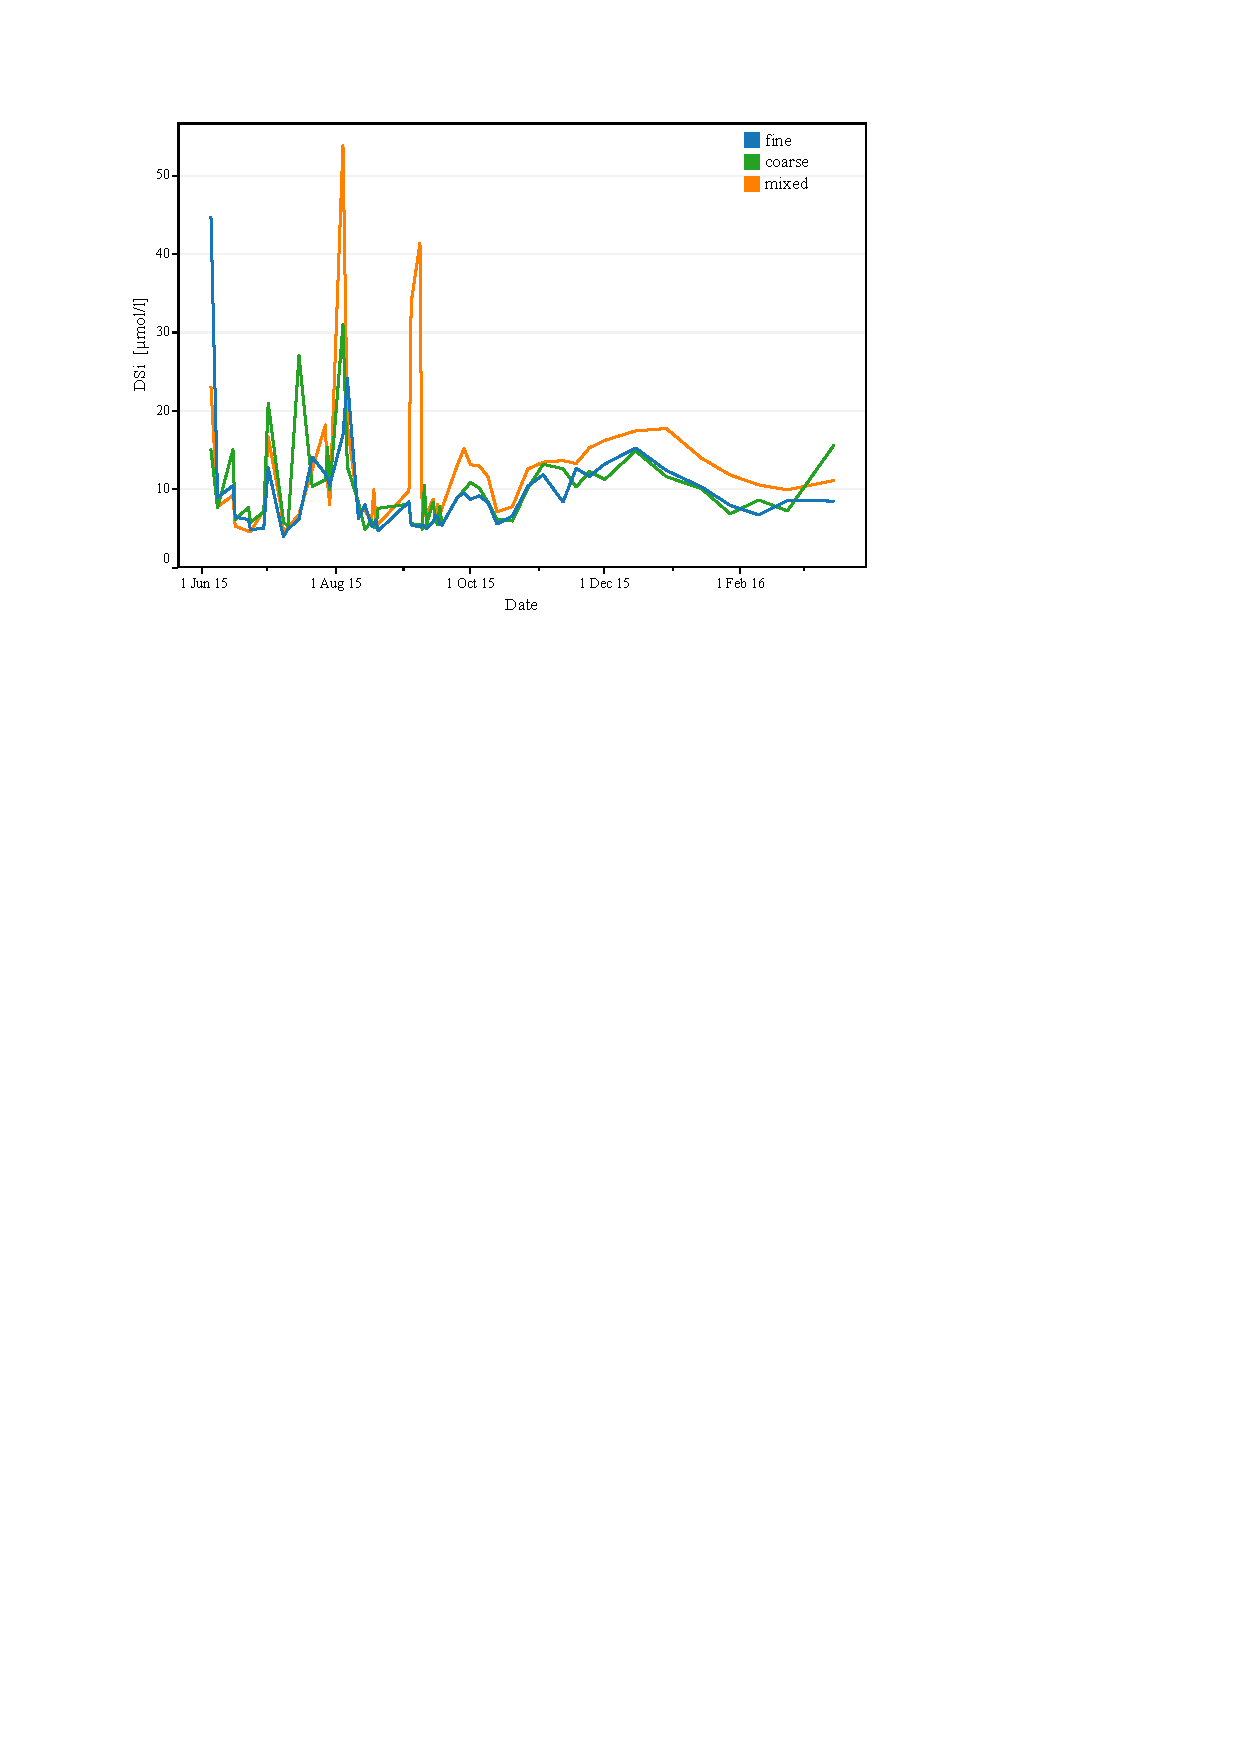
\includegraphics[scale=1]{dsi.pdf}
\caption{The outlet Dissolved Silica (DSi) plotted against Time (Date), averaged for the three grain types- fine, coarse, and mixed.}
\label{fig:results_dsi}
\end{figure}

\noindent \textbf{DSi:} The outlet silica concentration is measured in terms of DSi \ce{Si(OH)4} (\Cref{fig:results_dsi}). Unlike \ce{Mg^{+2}} and Alkalinity, Si values show no significant trend. The last four months show less fluctuations compared to the first four months. Mixed particles release slightly more Si than fines or coarse, atleast in the last six months. In general, due to the high fluctuations it's best to say that the values stay within a range of \SIrange{5}{20}{\micro\mole\per\litre}. It may be of worth to point out that as the experiment progressed, white particles were observed at the base of the columns. The water seeping through the gap between the rhizon-hole and the rhizon flowed down the column, and overtime the water evaporated leaving the 'salts'/residue behind. Analysis of the residue showed presence of Silica. Thus, even though the outlet DSi values are low and thus the contribution of the Si outside might be significant, the total water seeping through the gaps is very small and the overall affect can be neglected. \\

\noindent \textbf{Mg/Si ratio:} The ratio of Mg to the Si release is useful in knowing the state of the system and mechanism of the reaction. As previously discussed in \cref{subsec:nonstochio} forsterite shows apparent non-stochiometric dissolution due to formation of a Si-rich layer on the mineral surface. The ratio of Mg/Si is plotted against Time (Date) in \Cref{fig:results_mgsi} for the three grain types. The ratio increases in the first month and then sharply decreases for fine and mixed grain-type while coarse particles show a smaller drop which occurs earlier. The last measured value is around \num{40}. A ratio of 1.88 would imply stochiometric dissolution (see \Cref{eq:results_olivine}) and steady state conditions. Therefore, the current system is still far from steady-state which is unlike past experiments where steady state and stochiometric dissolution was achieved within a few hundred hours\; \citep{hellmann2012,pokrovsky2000,wogelius1992}.

The observation that outlet concentration profiles of Mg and Alkalinity ($\sim$ \ce{HCO3^-}) are similar and [Alkalinity] > [\ce{Mg^{+2}}], follows from \Cref{eq:results_olivine}. For every mole of forsterite reacted, \SI{1.88}{\mole} of \ce{Mg^{+2}} and \SI{4}{\mole} of \ce{HCO3^-} are produced. Silica doesn't show a similar trend due to reprecipitation and formation of Si-rich layer on the mineral surface. The preferred dissolution of fines or sites of high energy density are responsible for the high initial concentrations across the grain-types, especially for fine and mixed, which contain a higher percentage of them. \\
\begin{figure}[h]
\centering
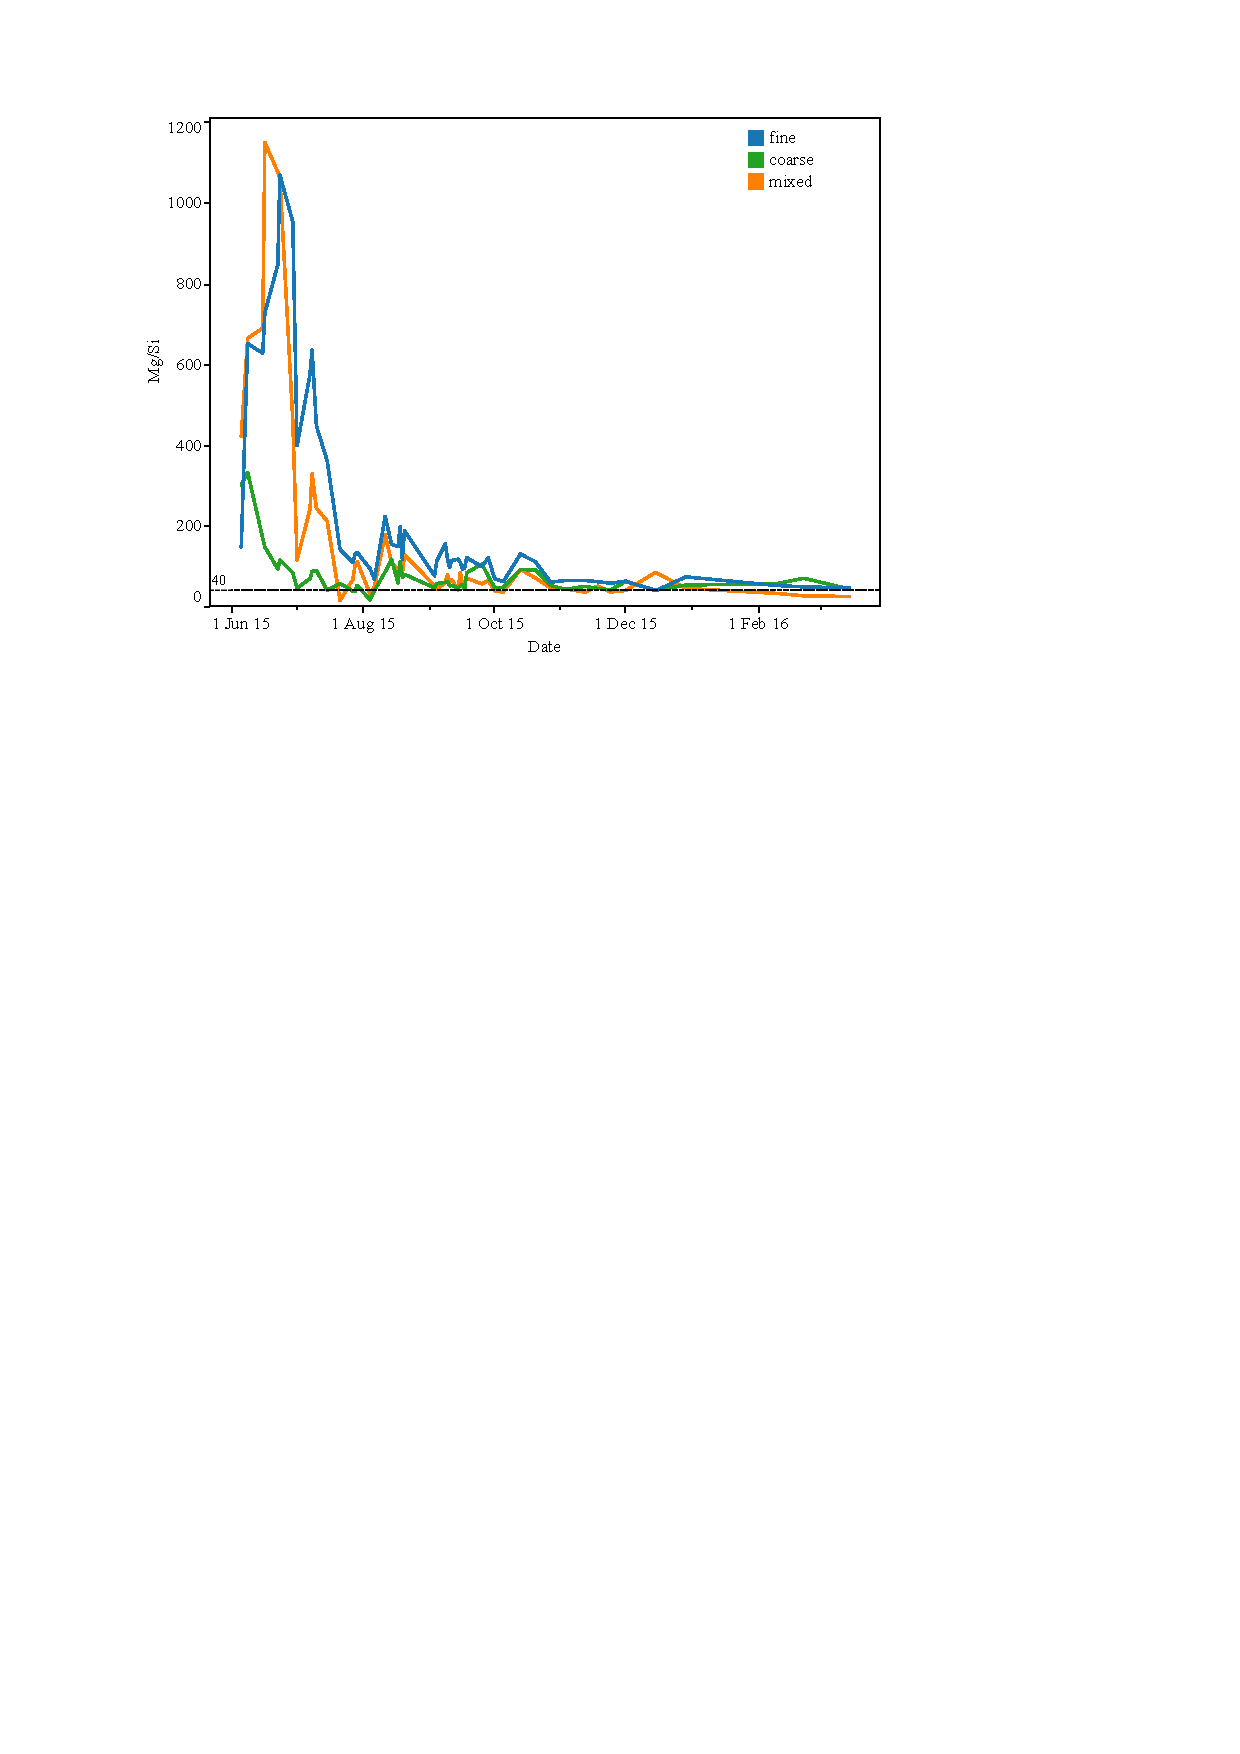
\includegraphics[scale=1]{mgsi.pdf}
\caption{The ratio of Mg/Si plotted against time and averaged for the three grain-types --- fine, coarse, and mixed.}
\label{fig:results_mgsi}
\end{figure}

\noindent \textbf{Minor ions:} The XRF analysis indicates the presence of other metal oxides in the olivine. These oxides are present inside other minerals like chabazite, hornblende, chlorite, lazardite \citep{marvin}. The elements in these minerals are also released in the solution, though in minor quantities. These minerals may have an effect on the overall dissolution rate because of different rates of dissolution (\citep{schott1981} in \cite{awad2000}). However, as forsterite is the dominant phase \citep{marvin}, and dissolves orders of magnitude faster than other minerals, the effect of the latter are expected to be insignificant (\citep{schott1985} in \cite{awad2000}). The concentration of minor cations with time - \ce{Na+}, \ce{K+}, \ce{Ca^{+2}} and minor anions - \ce{SO4^{-2}}, \ce{NO3-}, \ce{Cl-} is shown in\; \Cref{sec:app_minor_ion}.

\section{Thickness of `surface layer'}
The mechanism of formation of a Si-rich surface layer was discussed in \cref{subsec:nonstochio}. Mg and Si are released stochiometrically into the thin fluid layer surrounding the mineral but a part of the Si reprecipitates, leaving the other part as `observed Si' in the bulk solution. At steady state, the rate of release of `observed Si' equals the rate of precipitation so that the thickness of the Si-layer doesn't change. Past experiments give the thickness of this layer to be around \SIrange[range-units = single,range-phrase = --]{1}{5}{\nano\meter} \citep{hellmann2012,pokrovsky2000}. Calculations for the current experiment give the thickness in range of  \SIrange{0.2}{0.5}{\nano\meter} (see\; \Cref{sec:app_thickness}) depending on the grain-type. These results reveal that the system hasn't reached steady state, most of the Si-released is reprecipitated on the surface (leaving the `observed Si' to be very small), and the thickness ($T$) follows the order $T_{coarse}$ > $T_{fine}\; \sim\;T_{mixed}$.
\section{Pore volume and Residence time}\label{sec:results_pvrt}
The olivine contained in all columns occupied the same volume at the start of the experiment. The pore volume and porosity was calculated for each column, see \Cref{eq:pore_vol}, and is summarised in \Cref{tab:porosity}. 

\begin{align}
\begin{split}
\label{eq:pore_vol}
& V_l\;(\text{Pore volume}) = \text{Volume of cylinder containing olivine -  Volume of olivine}\\
& V\;(\text{Volume of cylinder}) = \pi \times r^2 \times h = \pi \times \mathrm{2.8^2} \times \text{20}=\SI{492.6}{cm^3}\\
& \text{Volume of olivine} = \textfrac{mass of olivine (column 1)}{density of olivine}=\textfrac{961.0}{3.32}=\SI{289.46}{cm^3}\\
& V_l = \num{492.6} - \num{289.46} = \SI{203.14}{cm^3}\\
& \text{Porosity} (\phi) = \textfrac{Pore Volume}{Volume of cylinder containing olivine}=\frac{V_l}{V}
\phantom{\hspace{0cm}}
\end{split}
\end{align}
\begin{table}[h]
     \begin{tabular}{cccc}
     \toprule
     \textbf{Column No.} & \textbf{Grain type} & \textbf{Pore Volume (\si{cm^3}) } & \textbf{Porosity} \\
     \midrule
     1 & coarse & 203.1 & 0.40 \\
     2 & coarse & 196.1 & 0.40 \\
     3 & coarse & 190.3 & 0.39 \\
     4 & fine & 302.8 & 0.62 \\
     5 & fine & 289.0 & 0.59 \\
     6 & fine & 293.8 & 0.60 \\
     7 & mixed & 217.5 & 0.44 \\
     8 & mixed & 227.2 & 0.46 \\
     9 & mixed & 218.9 & 0.44 \\
     \bottomrule
     \end{tabular}%
      \caption{Table showing the pore volume and porosity for different columns.}
   \label{tab:porosity}%
 \end{table}%

\noindent The pore-space or the pore-volume of a packed bed is the portion of the total volume that isn't occupied by the solid material \citep{nimmo2004}. The porosity ($\phi$) is fraction of the total volume taken up by the pore space. The porosity depends on the particle-size distribution, particle shape, and the absolute particle-size \citep{zou2011}. For particles smaller than \SI{\sim 100}{\micro\meter}, inter-particle forces, like vander-waals and electrostatic forces, become more important than gravity resulting in the formation of agglomerates or aggregates \citep{zou2011}. Thus, even though the porosity within these aggregates is small, the overall porosity of column is large due to agglomeration. This might explain why coarser particles have higher porosity than  fine or mixed grain type ($\phi_{coarse}$>$\phi_{mixed}$ > $\phi_{fine}$, see \Cref{tab:porosity}). 

The pore-volume is used to calculate the residence time (RT). The residence time, $\tau$ (seconds or days), is the average time spent by a water particle in a reservoir, and is calculated as the ratio of volume of reservoir to the flow rate of water. In column experiments with mineral dissolution, $\tau$ is the contact time between a mineral and a water sample. For the current experiment, the reservoir volume is the same as the pore-volume. The flow rate is calculated by dividing the outlet volume (water exiting from the column) by \SI{\sim 24}{\hour}\footnote{The water collected from the rhizons leads to fluctuations in the outlet volume. This water cannot be added to the outlet volume because it is forced out of the system. Since the rhizon sampling was done on specific days, one could remove the outlet volume from the following day in the calculation of residence time for consistency. This changes the residence time over the experiment duration, but the general trend is unaffected--- $\tau_{fine}$ increases the most, $\tau_{coarse}$ remains almost the same and $\tau_{mixed}$ shows an increase which is smaller than fine.}. The residence time is calculated, as an example, for column 1 (coarse); the outlet volume is taken for the month of March (see \Cref{eq:results_rt}). A similar calculation is performed for all months and grain-type and is plotted in \Cref{fig:rt}; the black line is the linear fit. It shows that absolute values of $\tau$ follow the order $\tau_{fine}$ > $\tau_{mixed}$ > $\tau_{coarse}$ at any point in time and  $\frac{d\tau_{fine}}{dt}$ > $\frac{d\tau_{mixed}}{dt}$ > $\frac{d\tau_{coarse}}{dt}$. \Cref{eq:results_rt} shows that $\tau$ depends on the pore-volume and the outlet flow rate ($F_l$). The development of $F_l$ with time (Date) is shown in \Cref{fig:results_fr}; the black line represents the linear fit. Assuming the pore volume to be constant with time, the higher initial $\tau$ for fine compared to coarse can be explained on the basis of the higher pore volume of fine compared to coarse (initial $F_l$ is almost the same), but as the experiment progresses, the changes in flow rate start playing an important role in shaping the residence time, i.e., a decrease in flow rate increases the residence time.
\begin{figure}[h]

\centering
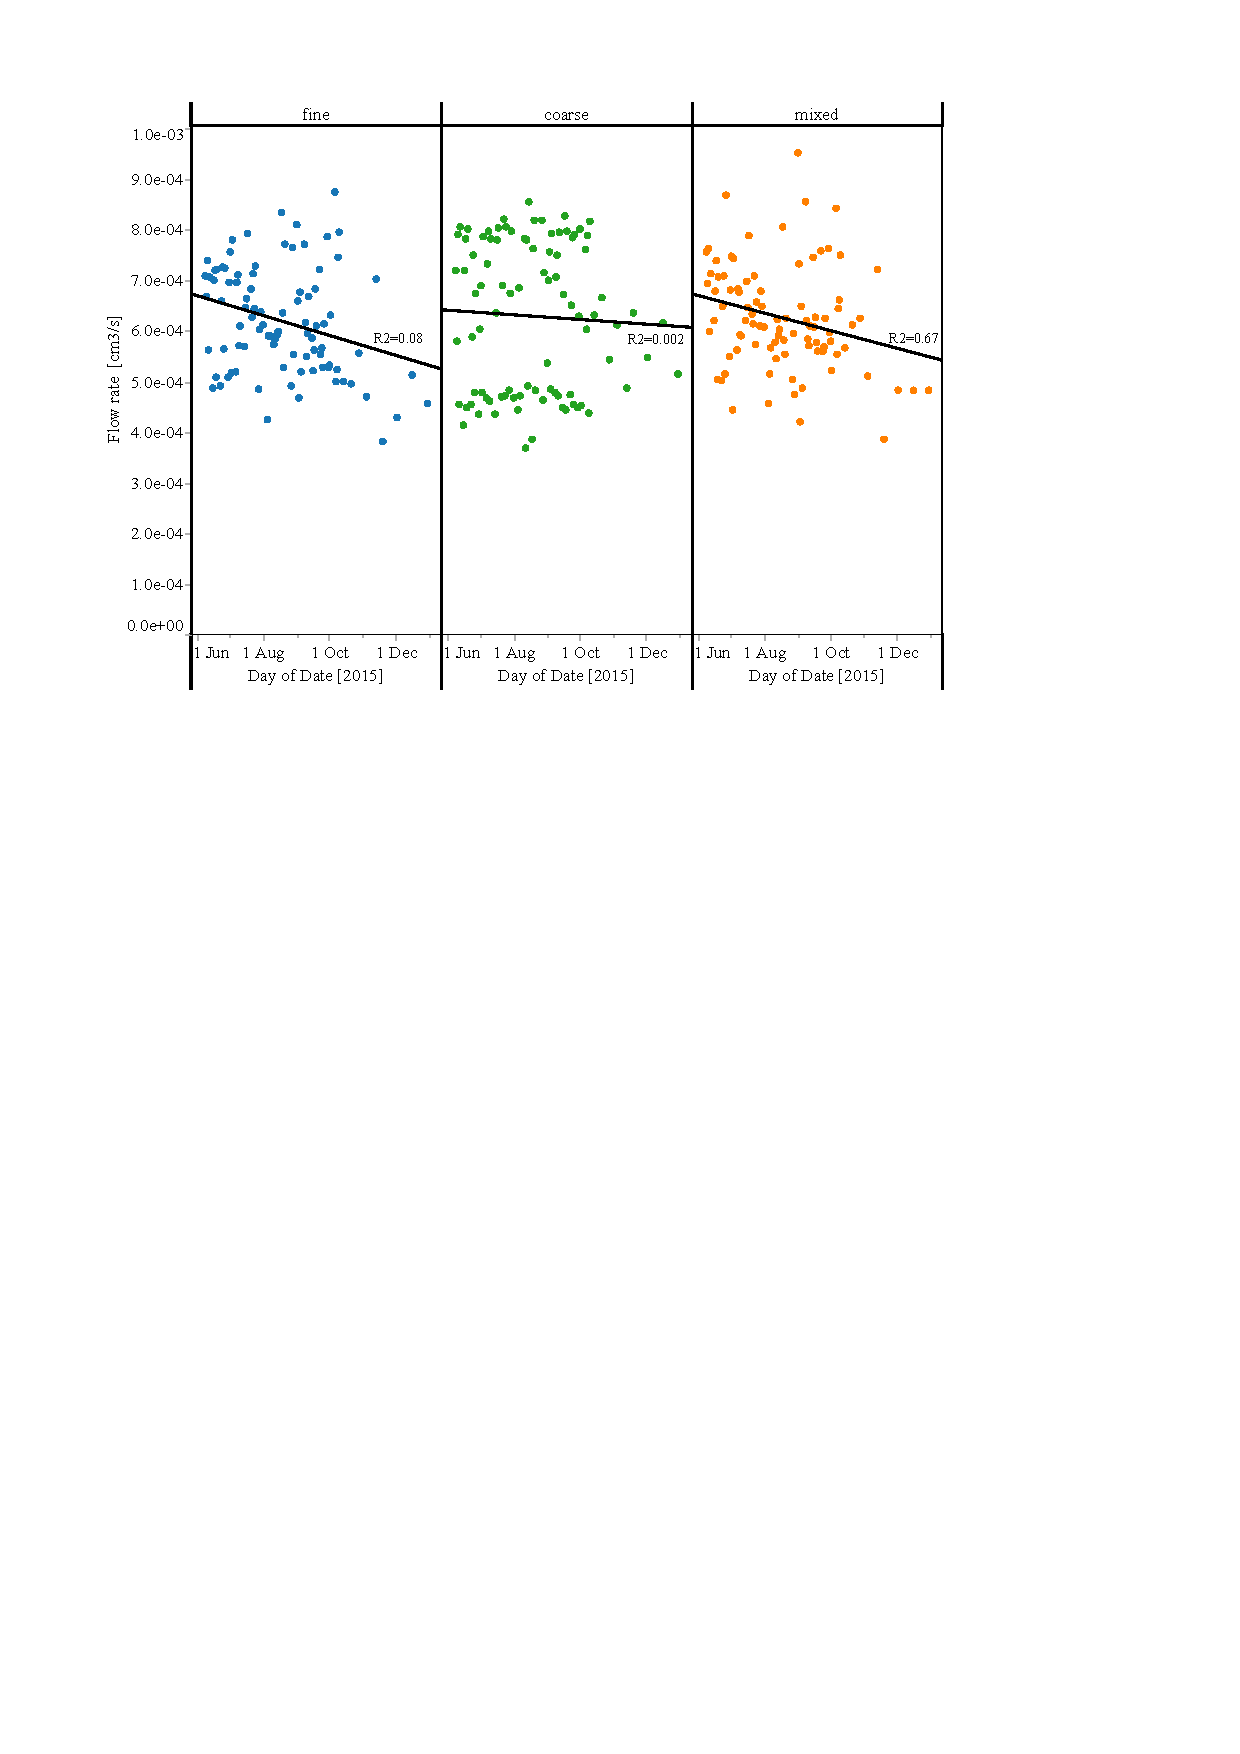
\includegraphics[scale=1]{flowrate.pdf}
\caption{Flow rate (\si{cm^3s^{-1}}) vs. Time (Date). The results are averaged for the three grain types- fine, coarse, and mixed. The black line is the linear fit. $R^2$ is the regression coefficient.}
\label{fig:results_fr}
\end{figure}


The changes in flow rate of the fluid are harder to quantify. The fluid flow velocity $u_c$ is calculated as flow rate divided by the cross-sectional area of the bed, and has been shown to depend on fluid viscosity, pressure difference across column, length of the column, porosity, surface of the column per unit volume of bed, specific surface area (per volume), tortuosity, and shape and size of particles\; \citep{coulson1991}. These factors are not further discussed  in this work.

\begin{equation}\label{eq:results_rt}
\begin{aligned}
F_l\;\text{(outlet flow rate)} &=  \textfrac{Outlet volume}{time}=\frac{\SI{68.21}{cm^3}}{(\num{24x 60 x 60})\si{s}}=\SI{7.9e-4}{cm^3.s^{-1}}\\
\tau &= \frac{V_l}{F_l} = \frac{\SI{203.14}{cm^3}}{\SI{7.9e-4}{cm^3.s^{-1}}} = \SI{2.57e5}{s}\\
\end{aligned}
\end{equation}

\begin{figure}[h]
\centering
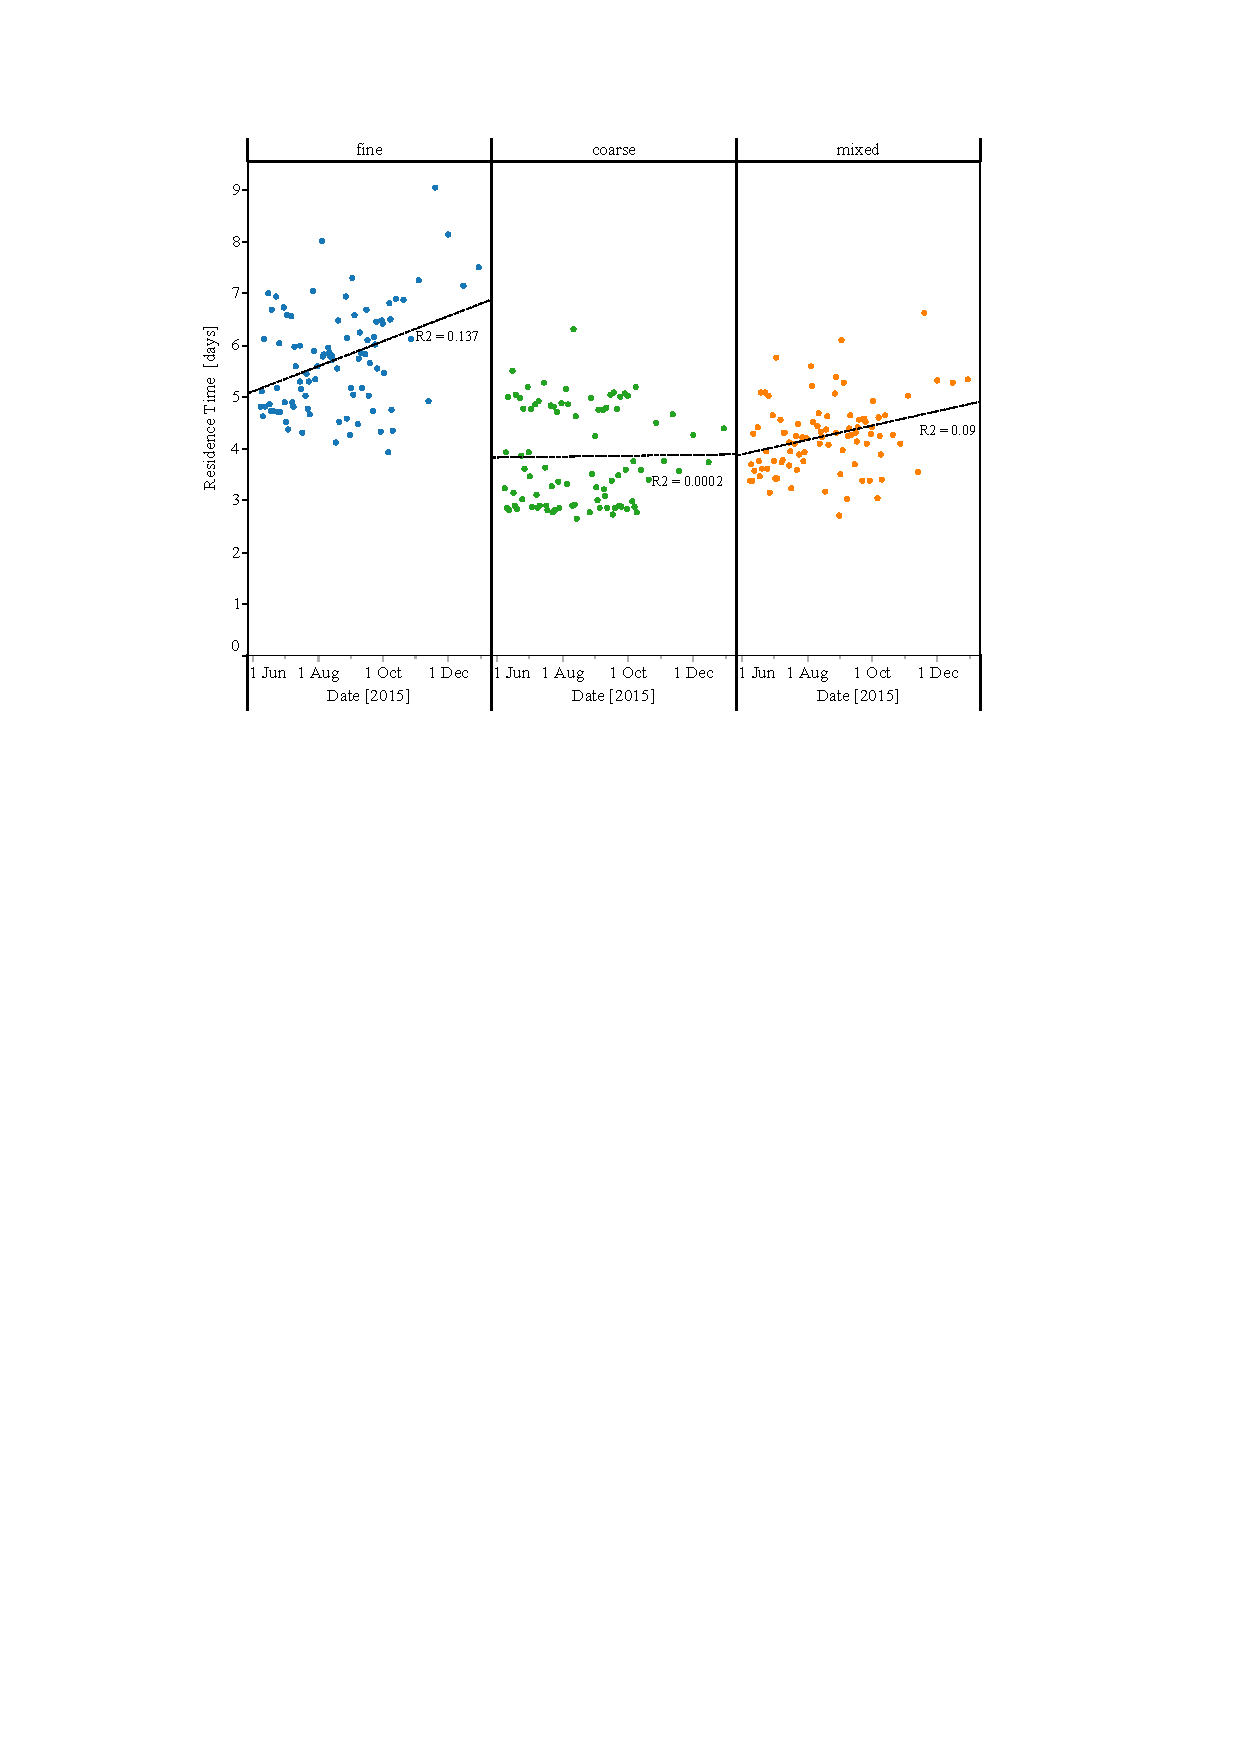
\includegraphics[scale=1]{rt.pdf}
\caption{Residence Time (days) plotted with the progress of the reaction (Date), for the three grain types--- fine, coarse, and mixed. The black line is a linear fit and shows the general trend. $R^2$ is the regression coefficient.}
\label{fig:rt}
\end{figure}

\section{Rate of Reaction}\label{sec:results_rate}
The reaction rate is calculated as the release rate of products into the solution. As an example, for column \# 1 and \ce{Mg^{+2}} (observed in March) the rate is calculated as:
\begin{align}\label{eq:rate_mg}
R_{Mg} &= \frac{[\Delta Mg]\times \text{outlet volume}}{\tau \times TSA}\\
R_{Mg} &= \frac{(\SI{546e-6}{\mole\per\litre}) \times (\SI{68e-3}{\litre})}{(\SI{2.57e5}{s}) \times (\SI{1018}{m^2})}=\SI{7.57e-14}{\mole\per\square\metre\per\second}
\end{align}

\begin{equation*}
\begin{aligned}
&\text{where,} \\
&\tau  = \text{residence time of water in column, \si{s}}\\
&TSA  = \text{Total surface area of particles, \si{m^2}} \\
&V_l  = \text{Pore volume}, \si{\litre}\\
\end{aligned}
\phantom{\hspace{6cm}}
\end{equation*}

\begin{figure}[h]
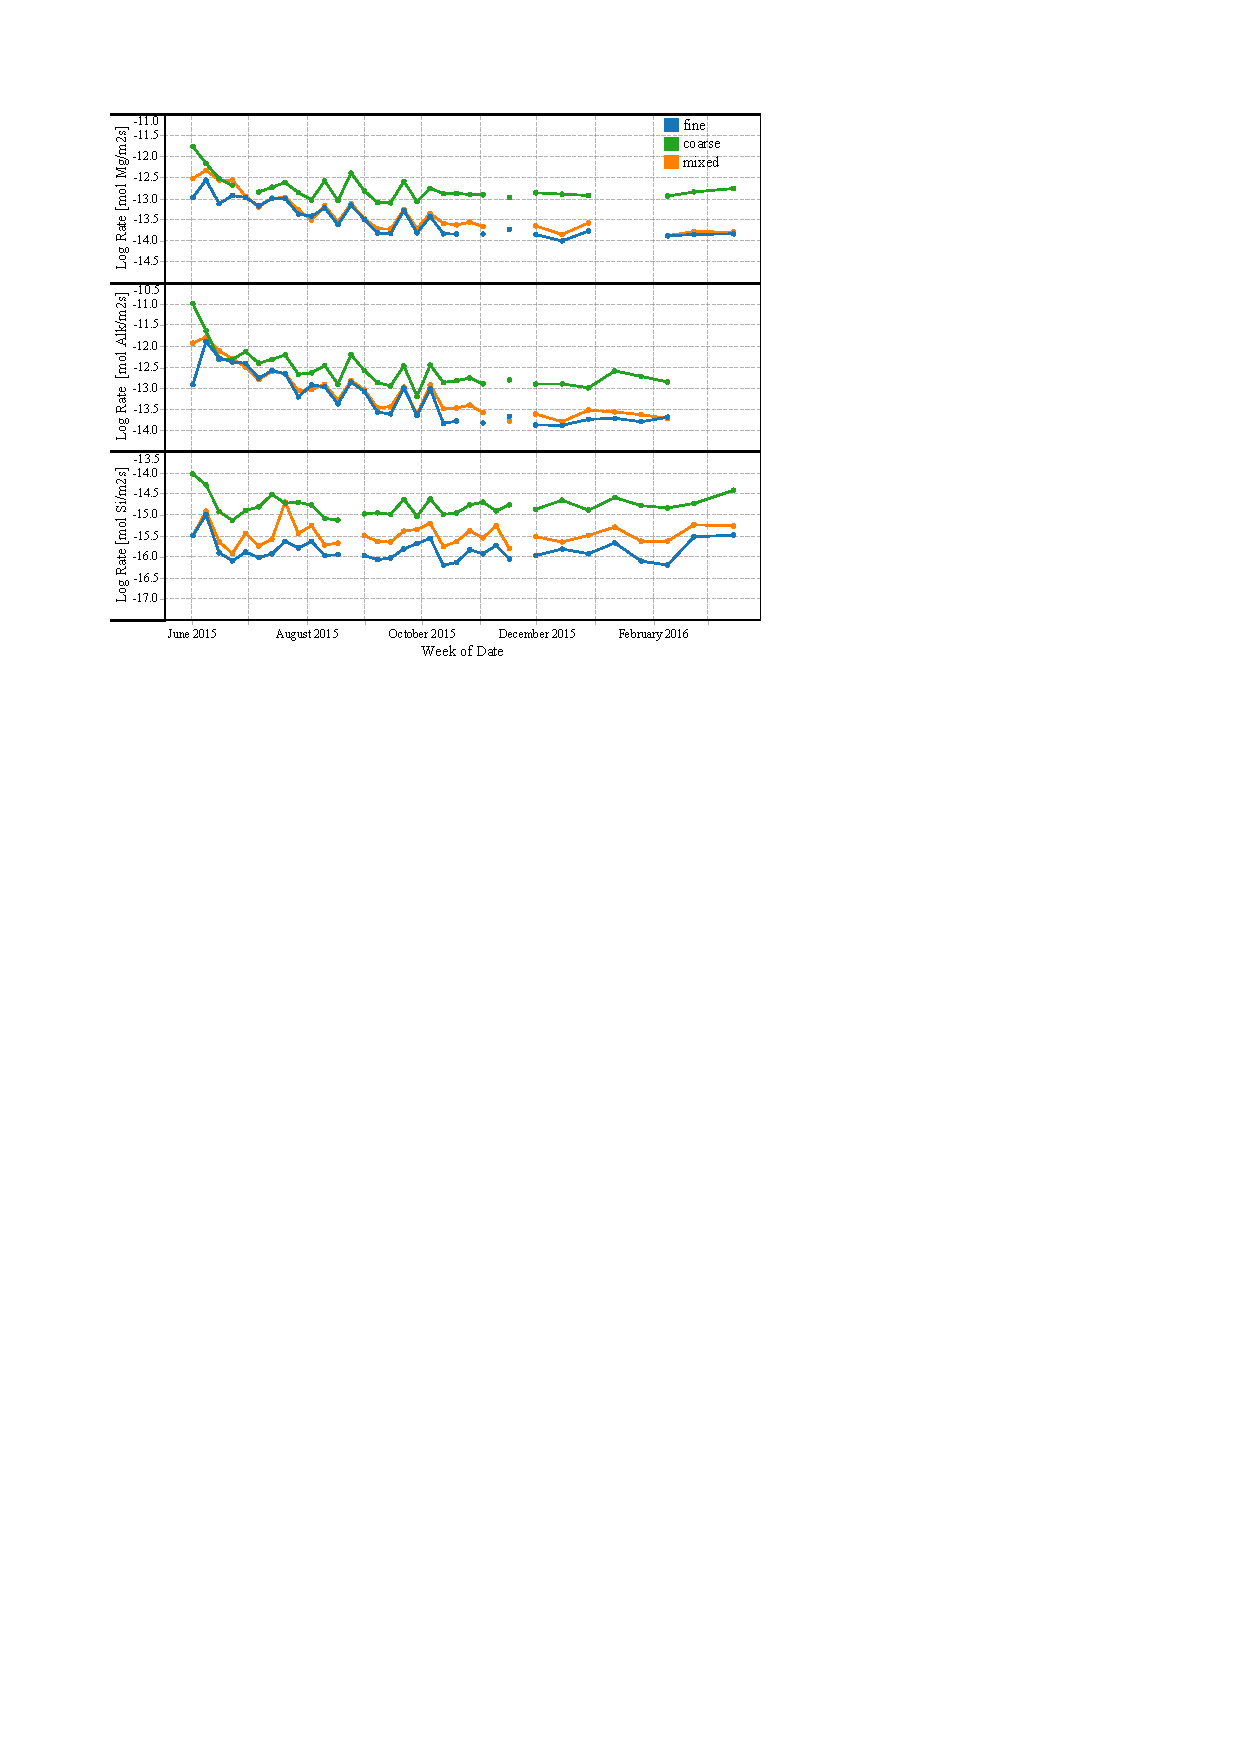
\includegraphics[scale=1.3]{rate.pdf}
\centering
\caption{The rate of reaction in terms of Mg, Alkalinity, and DSi (in \si{\mole\per\square\metre\per\second}) plotted against Time (Date), averaged for the three grain types--- fine, coarse and grain and over week.}
\label{fig:rate_Mg_al_si}

\end{figure}

\noindent The rate of release of Alkalinity and DSi is similarly calculated. The combined results are shown in \Cref{fig:rate_Mg_al_si}. In general they follow a trend similar to that of concentration (see \Cref{fig:results_mg1,fig:results_alk,fig:results_dsi}). $R_{Mg}$ and $R_{Alk}$ decrease with time, for all grain-types. The decrease is fastest in the first four weeks of the experiment. $R_{DSi}$ shows no particular trend and seems to stay between a range of values. The rate of reaction measured for Mg, Alkalinity, and DSi follows the order: $R_{Alk} \sim R_{Mg}$ > $R_{Si}$. The rate of reaction is higher for coarser particles than fine particles, and fine and mixed particles show similar values, i.e., $R_{Mg_{coarse}}$>$R_{Mg_{fine}}\sim R_{Mg_{mixed}}$. A similar observation is seen for $R_{Alk}$ and $R_{Si}$.\\

The decrease in $R_{Mg}$ and $R_{Alk}$ (see\Cref{fig:rate_Mg_al_si}) could be explained by two separate factors. Intrinsic factors are related to the physical and chemical properties of the mineral and how they change with time. These factors are enclosed within $TSA$ in \Cref{eq:rate_mg}. The decrease in reaction rate with time, observed in previous experiments, has been attributed to the fast dissolution of fine particles or sites of high surface energy \citep{Brantley2008b}. The olivine rock in this work also contains fines and sites of high energy density (created during grinding and crushing) and thus, their fast dissolution too could partly provides an explanation. Furthermore, BET surface area measured, for fine grains, one year after the start of the current experiment show a \SI{\sim 15}{\percent} increase in surface area (\Cref{tab:BET_a_table}). \cite{white2003} in long-term columns experiments with granite suggested that at-least a third of the decrease in their observed reaction rate with time was due to increases in physical surface area. In conclusion, intrinsic factors- reduction in energetic sites and increase in physical surface area, at least partly contribute to the decrease in reaction rate with time. Extrinsic factors, on the other hand, like hydrology, solute composition are external to the silicate mineral and are more difficult to understand \citep{white2003}. In \Cref{eq:rate_mg}, these terms are $\Delta$Mg, residence time $\tau$, and outlet volume. As shown and discussed in the previous section, in general, $\tau$ increases with time, [\ce{Mg^{+2}}] decreases with time, and outlet volume decreases with time ($F_l$ is outlet volume divided by time). When these effects are considered independent of each other they could also explain the observed decrease in reaction rate. In summary, both intrinsic and extrinsic factors control reaction rate though the relative importance of each cannot be exactly quantified.

Another reason could be the flushing out of particles from the column (\SI{<20}{\micro\metre}) (the aperture of the nylon sieve at the bottom of the columns is \SI{20}{\micro\metre}), or their complete dissolution in the initial phase. Since these particles contribute to a significantly to the rate, the escape or reduction of a tiny fraction could lead to a reduction in overall rate. No tests were unfortunately performed to find this. 

\noindent It is also observed in \Cref{fig:rate_Mg_al_si} that $R_{Mg}$ is almost two orders of magnitude greater than $R_{DSi}$.  The difference in release rates during silicate dissolution can be due to incongruent or non-stochiometric dissolution, difference in stochiometric amounts of elements present in minerals, or both \citep{rimstidt2012}. The different release rates in this experiment are because of the apparent incongruent dissolution due to formation of a surface layer (see \cref{subsec:nonstochio} for explanation and almost all Si released is precipitated - \Cref{tab:results_thickness}) as well as the different stochiometric contribution (see \cref{eq:results_olivine}). The large difference in rates means that the former process dominates.

\noindent The columns with coarser grain-type show almost an order of magnitude higher reaction rate than fine and even mixed grain-type (see the average over last months in \cref{fig:rate_Mg_al_si}). Generally at any time t, $\Delta\mathrm{Mg_{fine}}$ > $\Delta\mathrm{Mg_{coarse}}$, $F_{l,fine}$ < $F_{l,coarse}$ ($F_l$ is taken as proxy for outlet volume), $\tau_{fine}$ > $\tau_{coarse}$, $TSA_{fine}$ > $TSA_{coarse}$. The first two terms are directly proportional to rate while the last two are inversely proportional to rate. Thus, if the absolute difference in Mg is not higher than the absolute differences of $F_l$, $\tau$, and $TSA$, coarse particles would have a higher rate than fine particles. 

\subsection{Rate comparison with literature}
 
The observed reaction rate is compared with previous forsterite dissolution experiments. The compilation of previous experiments at \SI{25}{\degreeCelsius} was done by \cite{rimstidt2012}. They summarise that almost all past experiments reached congruency and steady-state, therefore, the difference in release rates of Mg and Si were only due to stochiometry effects. \Cref{fig:comparison} shows the plot of $R_{Mg}$ from \cite{rimstidt2012} normalised to BET surface area) against pH. To get an estimate of the rate difference, the past rate data is compared at pH 8 (see \cref{fig:results_ph}) with $R_{Mg},\; R_{Alk},\; R_{DSi}$ from \cref{fig:rate_Mg_al_si}, even though the current experiment hasn't reached steady state. The latter are averaged from the last few months of the experiment. A range of the rate is presented to account for the difference across columns/grain-types. The upper and lower bounds are coarse and fine grain-type respectively. Thus, depending upon which element and which grain type is taken, $R_{Mg},\;R_{Alk}$  are \num{\sim 3} orders of magnitude, and $R_{DSi}$ is \num{\sim 4} orders of magnitude smaller than past experiments.\\
 
\begin{figure}[h]
\centering
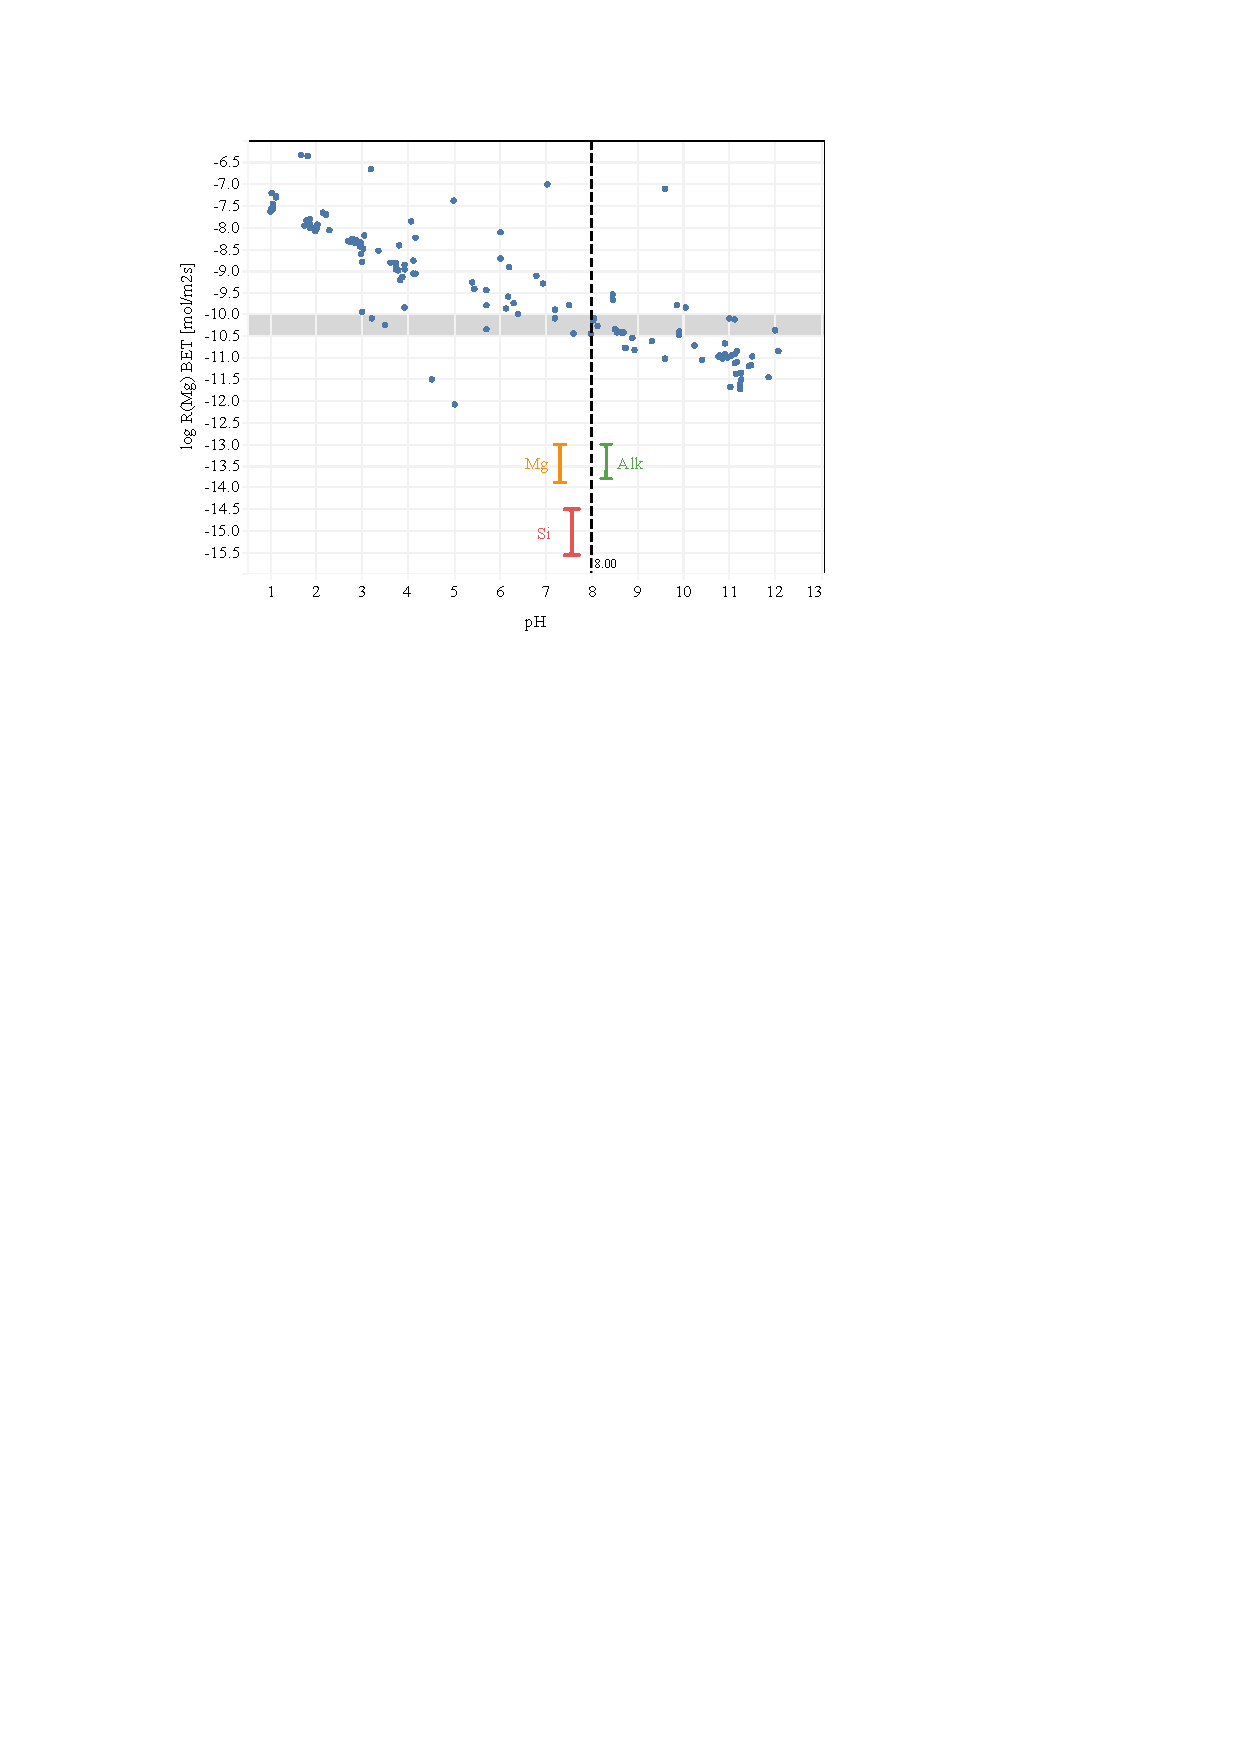
\includegraphics[scale=1.3]{comparison.pdf}
\caption{Rate data (in terms of log $r_{BET}$ \ce{Mg^{+2}}) vs. pH from past experiments on forsterite dissolution \citep{rimstidt2012}. The black line is the pH of interest. The range of  Mg, Alkalinty, Si rates shown in orange, green, and red respectively.}
\label{fig:comparison}
\end{figure}

Past dissolution experiments were conducted under similar conditions in closed MFRs and BRs - at \SI{25}{\degreeCelsius}, with very low rock to volume ratio, pre-treatment of grains to remove fines, sample containing almost uniform grain-size, and run time of few hundred hours. The current experiment on the other hand is a column experiment, with high-rock to volume ratio conducted without pre-treatment to remove fines, and rates observed over long time period. Thus, the comparison of reaction rate with literature is only possible when common factors affecting rate have been proven to not have influenced the rate. The factors affecting rate in surface-controlled reactions were discussed before in \cref{subsec:factors}.
 
\begin{enumerate}
\item \textbf{pH and temperature}: Unlike previous laboratory experiments which control system pH by changes in concentration of acids like \ce{H2SO4} or \ce{HCl} (see Table 1, \citep{rimstidt2012}), no such control was done in this experiment. The inlet water (in equilibrium with the atmosphere and at pH 5.7) is assumed to immediately turn alkaline upon contact with the first layer of olivine and remain constant throughout the column. This assumption is supported by previous experiments where a reactor containing water immediately turned alkaline upon addition of few grams of olivine \citep{martinez2014,dessen2016}. Assuming the conditions in column to have a higher pH, say 9 (which lead to lower rate, see \cref{fig:comparison}) one cannot still explain the large difference observed between observed and past values.\\

\begin{figure}[h]
 \centering
 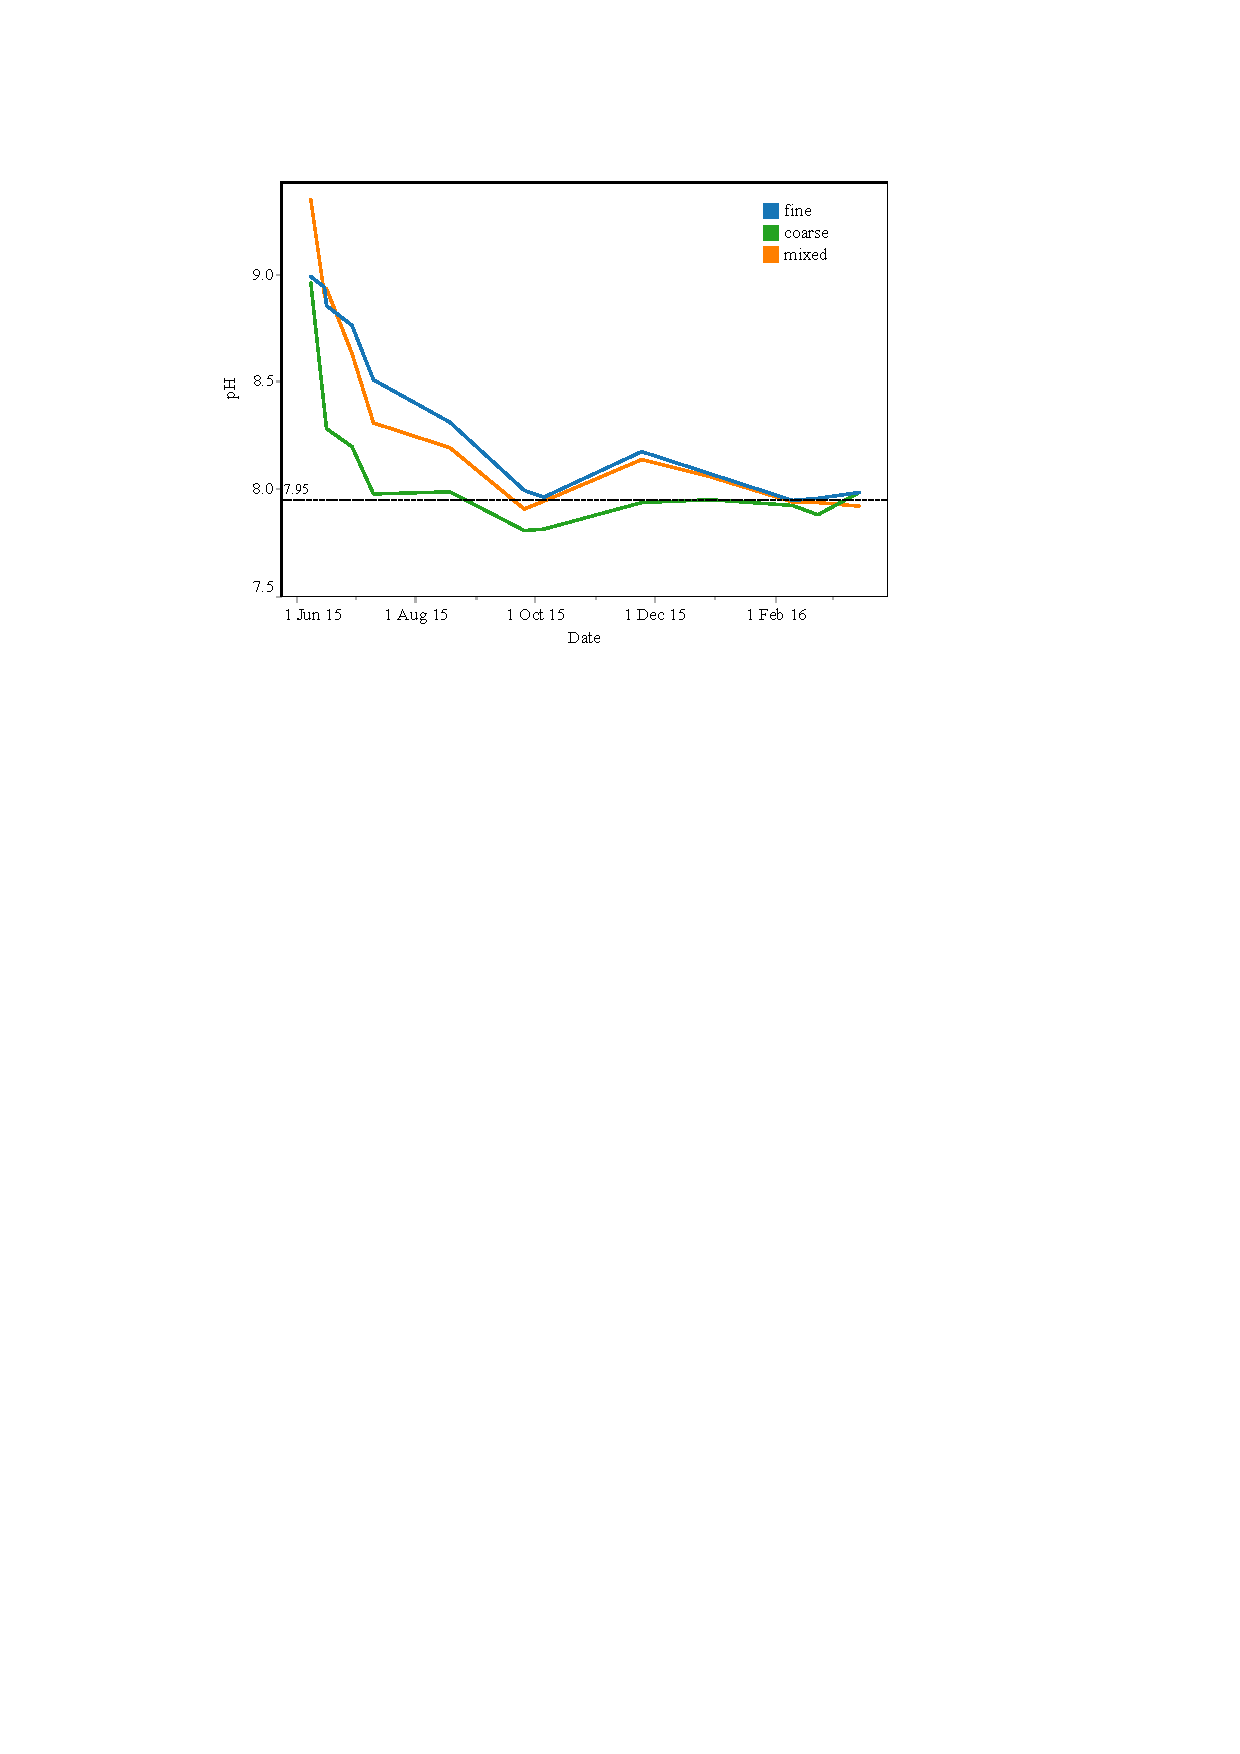
\includegraphics[scale=1]{pH.pdf}
 \caption{pH of the outlet water plotted against Time (Date) for the three grain types --- fine, coarse, and mixed.}
 \label{fig:results_ph}
 \end{figure}
 
\noindent The effect of temperature on reaction rate is found by using \Cref{eq:rimstidt}. The rate difference at \SI{20}{\degreeCelsius} and \SI{25}{\degreeCelsius} is \num{\sim 0.1} log units. Thus, even assuming the experiment temperature to be a few degrees lower than \SI{25}{\degreeCelsius}, it alone cannot explain the difference.

\item \textbf{Total surface area}: The contribution of the ultrafine grains (\SI{<10}{\micro\meter}) to the specific surface area is almost \SI{97}{\percent} and \SI{90}{\percent} for the  coarse and fine grain type respectively (see \Cref{sec:BET_a}). \Cref{sec:results_rate} discussed the  possibility of losing these ultrafines. Only one BET measurement was performed one year after the start of the experiment; the sample taken from the top of the column. This indicated an increase in SSA and would point that no ultrafines were lost during the experiment. Even though this result could be different for particles closer to the very end of the column, this effect is assumed to be small compared to the total column.

Most dissolution experiments are performed in MFRs and BRs, with agitators moving few grams of the mineral in a fluid medium. This wets the entire mineral surface and all grains are more or less equally wetted. The `wetted area' can be defined as the area of the mineral in contact with the fluid. In column experiments with high rock to volume ratio, neither the complete surface of a single grain nor different grains are uniformly wetted. This could be due to many factors - formation of dead zones (regions where water remains stagnant or doesn't reach at all), preferential flow (water seeps through fractures and cracks without interacting with many grains), compression and stacking of particles, and aggregation of fine particles. When BET values are used, unaccounting for these factors could lead to overestimation of the `actual and available surface area'. This is different from assuming the effective surface area to be same as BET surface area (see \cref{subsec:factors}). In fact, the concept of wetted surface area brings another layer of complexity in finding the `actual surface area' which takes part in the reaction.\\

Assuming the `actual surface area' to be, say, 20 times smaller than BET surface area, would lead to a 1.3 log units reduction in measured rate, and thus this factor alone cannot account for the observed rates. \\

\item \textbf{Effect of reaction products, p\ce{CO2}}
As already discussed, the concentration of reaction products or dissolved \ce{CO2} don't significantly or conclusively lead to change in dissolution rate. 

\end{enumerate}
Any of the factors taken alone cannot explain the observed dissolution rates. Even assuming a combination of the higher end of rate values for each factor, it wouldn't explain more than half of the difference observed. Thus, common factors that usually influence surface-controlled rate don't explain the observed results. Furthermore, a surface-controlled rate would mean that the rate is independent of particle size, which is contradictory to observation. These results leave the possibility of the reaction rate to be transport-controlled or a mixture of transport and surface control, and will be discussed in the next section.  

\subsection{Transport control in column reactors}
To get an estimate of the reaction rate in a packed bed and of forsterite and the factors controlling it, a theoretical model of \cite{rimstidt2015} is used. This model includes diffusion and surface reaction equations. Before the reaction occurs at the mineral surface, the reactant, \ce{H+} ions, must move from the bulk of the fluid across a static thin fluid film to the surface. This movement, called diffusion flux, is driven by the concentration gradient across the film. The values of the diffusion flux ($J_D$) and reaction flux ($J_R$) decide what controls the overall reaction rate. Both are calculated normalised to geometric surface area. The model thus explores how mineral dissolution in a packed bed is affected by flow rate, grain diameter, diffusion coefficients, and temperature \citep{rimstidt2015}. The equations for $J_D$ and $J_R$ are given in \Cref{eq:results_diff}.
\begin{equation}\label{eq:results_diff}
J_D=k_D(c_s-c)
\end{equation}
\begin{equation}
J_R=-k_Rc_s
\end{equation}

where $k_D$ is the diffusion coefficient, $c_s$ is the [\ce{H+}] at the surface, $c$ is the bulk [\ce{H+}], $k_R$ is the rate constant of the reaction. 

The diffusion coefficient is further defined as:
\begin{equation}\label{eq:results_kd}
k_D=\text{1.17}\;{\left( \frac{Lq}{\nu}\right)}^{\text{-0.42}}{\left( \frac{D}{\nu}\right) }^{\textfrac{2}{3}}
\end{equation}

where $L$ is the particle diameter (m), $q$ is the Darcy velocity (\si{\metre\per\second}), $\nu$ is kinematic viscosity (\si{\square\metre\per\second}), $D$ is the diffusion coefficient of the aqueous species (\si{\square\metre\per\second}).

The model is slightly modified to account for the higher pH in the current experiment (Rimstidt only showed results for pH \num{<5.6}). The model rates are steady-state in terms of the reactant, \ce{H+}, and have been modified through stochiometry to obtain release rates of products --- \ce{Mg^{+2}} (adding log 0.5 = - 0.3 to \ce{H+} release rates) and Si (addding log 0.25 = - 0.6 to \ce{H+} release rates). The model doesn't acccount for p\ce{CO2} affects. The variables entered into the model are summarised in \Cref{tab:results_rimstidt_model}. The Darcy velocity, $q$, is the volumetric flow rate divided by the cross-sectional area transited by the flow. The grain diameter, $L$, is taken as the mean of the grain size distribution obtained by laser-granulometry. \\

 \begin{table}[h]
   \centering
     \begin{tabular}{cccc}
     \toprule
     \textbf{Grain type} & \textbf{Darcy velocity, $q$ (\si{\metre\per\second})} & \textbf{Grain diameter, $L$ (\si{\micro\meter})} & \textbf{pH} \\
     \midrule
     Fine & \num{2.8e-7} & 25 & 8 \\
     Coarse & \num{1.68e-5} & 680 & 8 \\
     \bottomrule
     \end{tabular}%
     \caption{Variables pertaining to the current experiment entered into the model of \cite{rimstidt2015}.}
   \label{tab:results_rimstidt_model}
 \end{table}

The results are summarised in \Cref{fig:results_rimstidt}. At the temperature of interest $J_D << J_R$ by almost four orders of magnitude. Thus, the reaction rate is diffusion-controlled. Further, coarse particles have a higher (0.5 log units) rate than fine particles which is due to different  particle diameter and Darcy velocity (see\;\Cref{eq:results_diff,eq:results_kd}).

\begin{figure}[h]
\centering
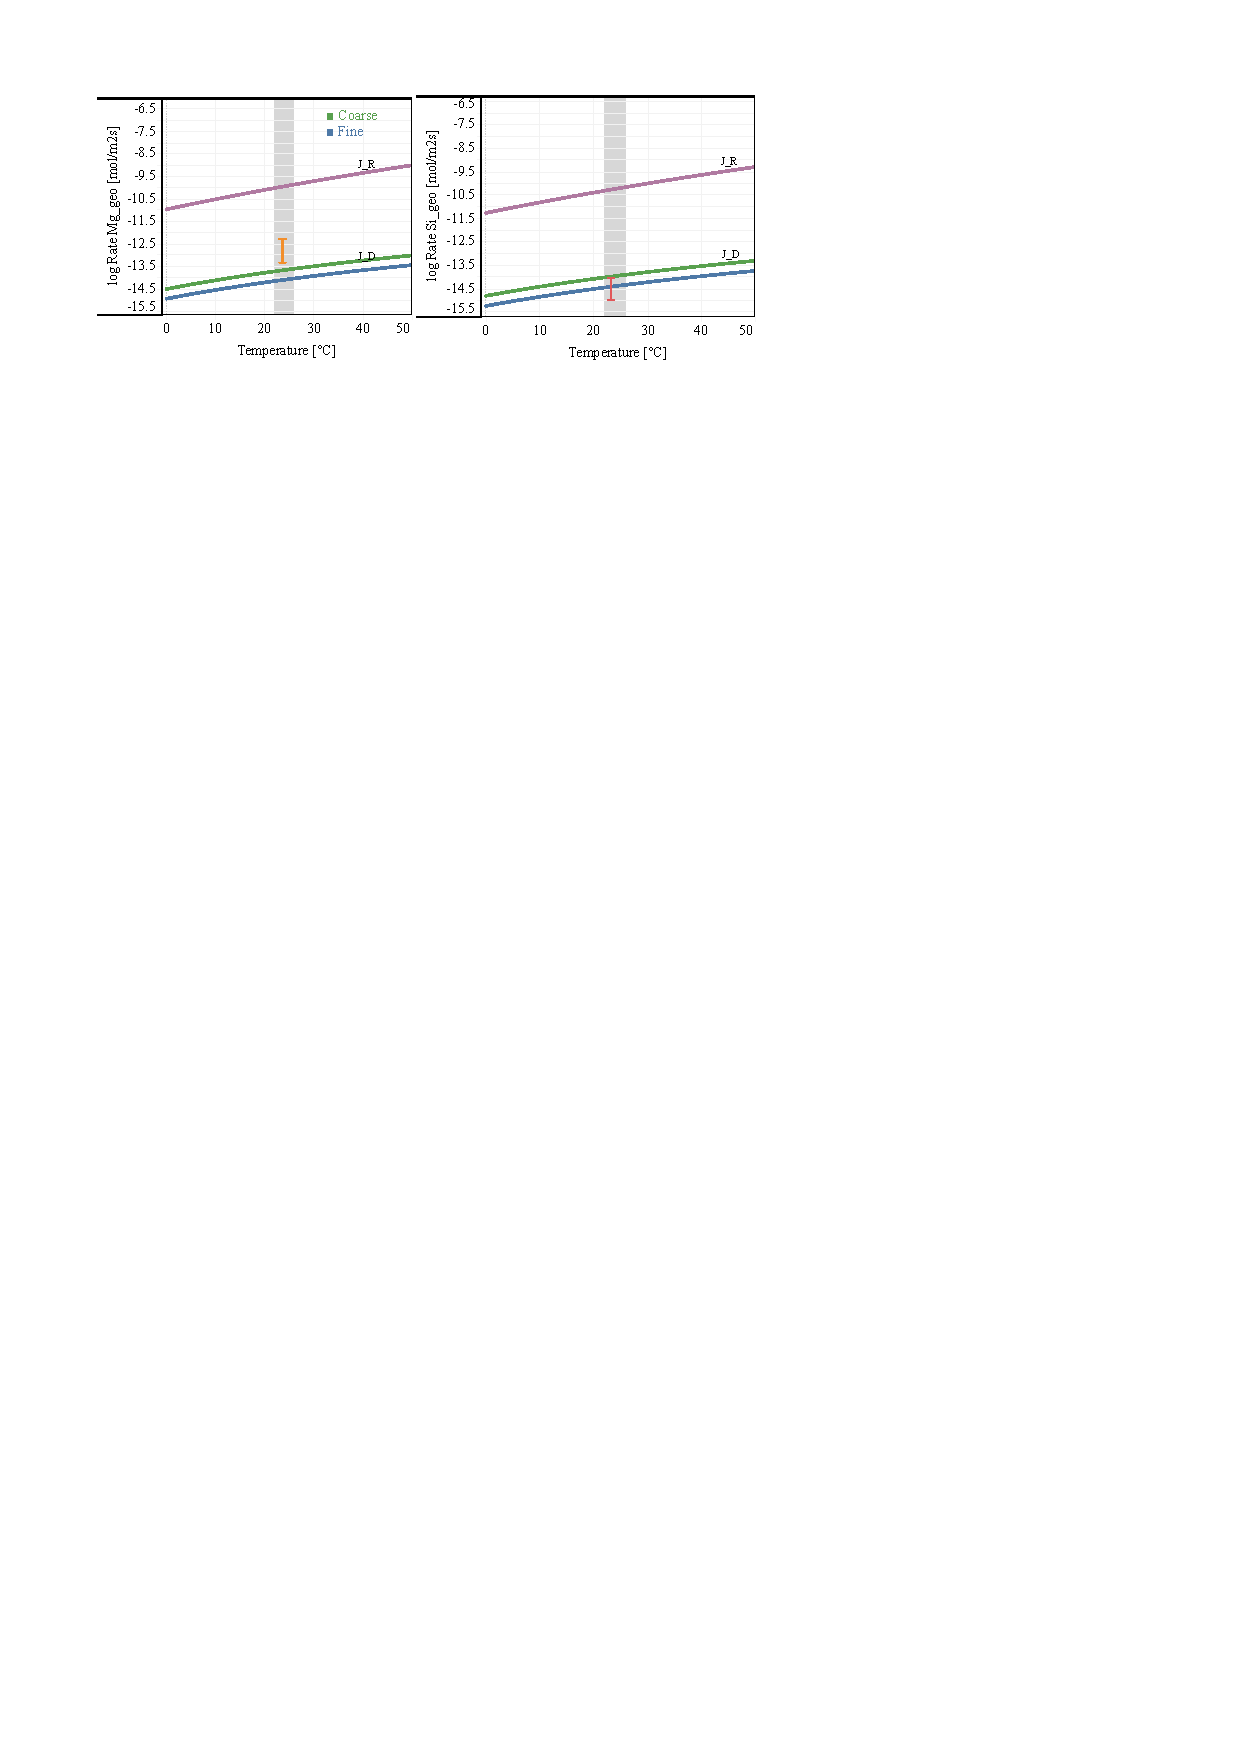
\includegraphics[scale=1.3]{rimstidt.pdf}
\caption{Plot of Log Rate of dissolution (in \si{\mole\per\square\metre\second}), vs. Temperature (\si{\degreeCelsius}) at pH 8. The purple curve is the reaction flux ($J_R$) and is the same for fine and coarse grain types. $J_D$ is the dissolution flux for fine (green) and coarse (blue). The green and red bar are the range of measured values for Mg and Si respectively. The grey band is the temperature range of interest.}
\label{fig:results_rimstidt}
\end{figure}

In order to compare the model and experimental results, the BET normalised surface rates of the experiment are converted to geometric surface rates by dividing the former by a factor of 5 (or adding 0.7 log units to the rate term in \Cref{eq:rate_mg}) (see \cite{rimstidt2012} for discussion on roughness factor). The rates are presented as a range due to difference in rates across grain-type. The experimental rate is about one to two orders of magnitude larger than model results for Mg but almost the exact range for Si (\Cref{fig:results_rimstidt}). It's worth mentioning that the current experiment hasn't reached steady state while the model results assume steady-state. This means that experimental results will decrease in the future though extremely slowly.


Another process could explain the one to two order difference, between experimental and model results, observed for Mg. As each column is watered, the water doesn't immediately trickle down the column but stays at the top for some time. The amount and time of this over-head water increased as the experiment progressed. This means that the thin layer, a few grams, of olivine at the very top may react faster (with a value $J_R$) than the rest of the column because it is in contact with a comparatively large amount of water. This could explain the higher rate observed for Mg. A corresponding higher rate is not observed for Si because of the formation of a Si-rich layer around the mineral surface. 
